\chapter{Plan del proyecto}\label{ch:primer-capitulo}
\section{Definición de las tareas a realizar}

Este capítulo describe la planificación del Trabajo Fin de Grado realizado. Atendiendo a los objetivos mencionados en la introducción, se ha realizado el siguiente desglose en tareas: 
\begin{itemize}
    \item Tarea 1 (\textbf{T1}): En una primera toma de contacto con el artículo~\cite{chen1995universal}, esta tarea consiste en realizar una lectura identificando los puntos clave del mismo y revisando qué conceptos se conocen y cuáles no, con el objetivo de establecer un plan de estudio que nos permita llegar a comprender estos conceptos.
    \item Tarea 2 (\textbf{T2.1},\textbf{T2.2}): Comprende la adquisición de los conocimientos identificados durante la tarea anterior. Para ello, se ha visto conveniente realizar un estudio individual de la Teoría de Distribuciones (\textbf{T2.1}) acompañado de la asistencia como oyente al curso de Análisis Funcional Avanzado impartido en la titulación de máster FisyMat de la Universidad de Granada (\textbf{T2.2}).
    \item Tarea 3 (\textbf{T3}): Consiste en el desarrollo de los resultados presentados en el artículo~\cite{chen1995universal}, detallando y completando sus demostraciones.
    \item Tarea 4 (\textbf{T4.1},\textbf{T4.2}): En ella se engloban tanto la adquisición de conocimientos teóricos necesarios como la familiarización con las librerías de las que se va a hacer uso en el proyecto. Para ello, se prevee un acercamiento teórico (\textbf{T4.1}) al estado del arte en PINNs mediante el estudio de las publicaciones científicas más relevantes en el campo y de publicaciones más relevantes referentes a la librería SciANN, acompañado de unas pruebas iniciales (\textbf{T4.2}) con las que se afianzarán los conocimientos adquiridos.   
    \item Tarea 5 (\textbf{T5}): Consiste en la definición y construcción del entorno experimental sobre el que va a realizarse la experimentación.
    \item Tarea 6 (\textbf{T6}): Se compone de las tareas de experimentación realizadas en el proyecto. Para cada tarea, se contempla el análisis del problema, el diseño del modelo de PINN asociado, la experimentación relativa a parámetros que definan el modelo y la evaluación de resultados. 
    \item Tarea 7 (\textbf{T7}): Recoge el proceso de redacción de la memoria del proyecto. 
\end{itemize}



\section{Planificación temporal del proyecto}

En la \autoref{tb:12} se muestra la planificación temporal estimada para el proyecto. Debido a la gran carga teórica previa, necesaria para comprender los resultados que se proponen en~\cite{chen1995universal}, las tareas de implementación (\textbf{T4.1} en adelante) no comienzan hasta abril, una vez los conocimientos teóricos que la fundamentan están asentados. Además, la \autoref{fig:img61} muestra cómo las fases teórica y de implementación ideadas se han visto solapadas durante el mes de abril, debido a la carga mencionada.
\begin{table}
    \resizebox{\textwidth}{!}{
    \begin{tabular}{|l|l|c|c|c|c|}
     \hline
     \multicolumn{6}{|c|}{\textbf{Desglose de tareas}} \\
     \hline
     \textbf{Tarea} & \textbf{Descripción} & \textbf{Duración} & \textbf{Inicio} & \textbf{Fin}& \textbf{Horas estimadas}\\
      \hline
     \ \textbf{T1} & Identificación de conceptos  & 1 semana &   21/08/2023 &28/08/2023 & 8\\ 
      \hline
     \ \textbf{T2.1} & Estudio de Teoría de Distribuciones  & 21 semanas &   04/09/2024 & 28/01/2024 & 130\\ 
      \hline
     \ \textbf{T2.1} & Asistencia a Análisis Funcional Avanzado  & 15 semanas&   26/09/2023 &16/01/2024 & 21\\ 
      \hline
     \ \textbf{T3} &  Desarrolo de demostraciones en~\cite{chen1995universal}& 13 semanas &   29/01/2024 &28/04/2024 & 80\\ 
     \hline
     \ \textbf{T4.1} & Estudio bibliográfico de PINNs  & 3 semanas&   01/04/2024 &21/04/2024 & 50\\ 
      \hline
     \ \textbf{T4.2}&  Pruebas iniciales complementarias  & 3 semanas&   01/04/2024 &21/04/2024 & 15\\
      \hline
     \ \textbf{T5} &Construcción del entorno experimental & 1 semana&  22/04/2024 &28/04/2024 &10\\
      \hline
     \ \textbf{T6}  & Experimentación & 7 semanas&   29/04/2024 &17/06/2024 & 100\\
     \hline
     \ \textbf{T7}  & Redacción de la memoria & 19 semanas&   01/04/2024 &10/07/2024 & 80\\ 
     \hline
    \end{tabular}
    }
    \caption{Desglose del proyecto en tareas.}
    \label{tb:12}
\end{table}

 \begin{figure}[htbp]
    \centering
    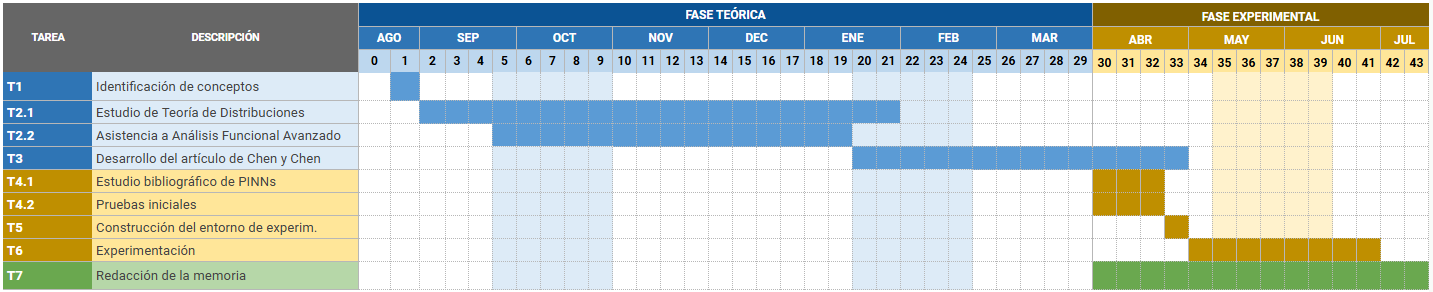
\includegraphics[width=1\textwidth]{img/img61.png}
    \caption{Diagrama de Gantt asociado al proyecto.}
    \label{fig:img61}
\end{figure}


\section{Estimación de coste}

Para la estimación del coste del proyecto, se han consultado distintas fuentes que garanticen una estimación fiable del precio por cada recurso. De acuerdo con el Informe de Tendencias Salariales publicado por la agencia de recursos humanos Randstad para el año 2023 \footnote{El informe puede consultarse en  \href{https://www.randstadresearch.es/tendencias-salariales/}{https://www.randstadresearch.es/tendencias-salariales/}.} , se estima que el salario medio de un Ingeniero de Software de rango medio en España es de 20\EUR $\backslash $hora. De acuerdo con la planificación temporal, se estima que se ha dedicado un total de 494 horas de trabajo. Esta cantidad de horas es superior a las que la normativa indica para el TFG de la titulación (18 ECTS).

Con respecto a los recursos necesarios para el desarrollo del proyecto, debe contemplarse la adquisición de ordenadores, con una estimación de $500$\EUR$\backslash $unidad, así como de subscripciones a Google Colab Pro+ ($51.12$\EUR$\backslash $mes), respetando así  el entorno de desarrollo del proyecto en este trabajo así como que se cuente con una capacidad de cómputo que garantice un una buena experimentación co modelos de aprendizaje profundo. Por último, sería conveniente el alquiler de un espacio de co-working que garantice un ambiente adecuado para el desarrollo del proyecto. El precio medio de alquiler de este espacio en Granada es de 130\EUR$\backslash $mes por empleado.


Dado que vamos a contar con un único empleado para realizar todas las tareas, se necesitaría un único recurso de cada tipo especificado durante un periodo de $11$ meses. En la \autoref{tb:141} se muestra el desglose del coste. 

\begin{table}[ht]
    \centering
    \begin{tabular}{|l|r|}
         \hline 
         \textbf{Recurso} & \textbf{Coste}\\
         \hline 
         Personal & 9.880\EUR\\
         \hline 
         Ordenadores & 500\EUR\\
         \hline 
         Subscripciones & 562,32\EUR\\
         \hline 
         %CAMBIAR COWORKING 
         Espacio de co-working & 1.430\EUR\\
         \hline 
         Total & 12.372,32\EUR\\
         \hline 
    \end{tabular}
    \caption{Coste estimado del proyecto.}
    \label{tb:141}
\end{table}

%\item Caso 2: Planteamiento de proyecto en equipo.

%De manera análoga, se propone contar con dos empleados para desarrollar el proyecto. Esto duplicaría el coste de los recursos de ordenadores, subscripciones y de espacio de co-working. Además, aunque las tareas \textbf{T4.2},\textbf{T5},\textbf{T6},\textbf{T7} puedan repartirse, hemos visto que el proyecto requiere de una componente de estudio bibliográfico que deberían realizar todos los integrantes del equipo para garantizar la fiabilidad de los resultados del proyecto. En la \autoref{tb:142} podemos ver los costes resultantes.  


%Aunque a través de las tablas mencionadas anteriormente se estima un incremento de coste del $60,67$\%, conviene remarcar que el trabajo en equipo suele dar mejores resultados y, por tanto, debería escogerse siempre que tengamos capacidad económica para ello. 